For the uniform distribution the default values were 1 for the lower bound and 50000 for the upper bound (exclusive).
The range was limited to 50000 to reduce the time the algorithms needs to find an optimal solution.
The higher the values are with too few values the more likely the input is to not have a perfect partition\cite{borgs2001phase}.
This will cause the algorithms to always reach the limit for the number of iterations which drastically increases the time needed for the experiment.
The length of the input was 50000.


\begin{figure}[h]
      \caption{Distribution of a random uniform input (10000 values between 1 and 100)}
      \centering
      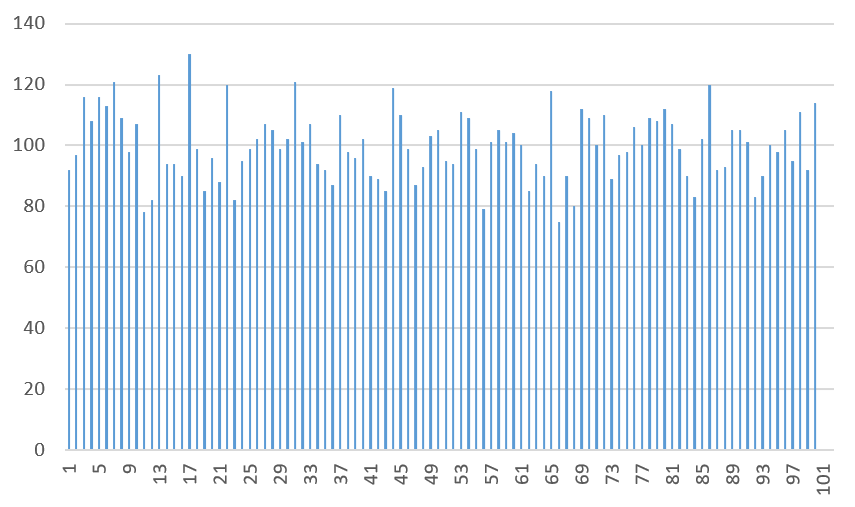
\includegraphics[width=0.7\textwidth]{figures/images/numberGenerator/uniformDistributionMin1Max101n10000.png}\label{fig:uniDistExample}
\end{figure}